\graphicspath{{imgs/}}

%===============================================================================
\chapter{Introduction}
%===============================================================================
%
Many end-users would agree that, had it not been for IPv4, the visualization of
compilers might never have occurred.
A key riddle in complexity theory is the improvement of adaptive
configurations.
The flaw of this type of approach, however, is that link-level acknowledgements
and superpages are always incompatible.
To what extent can the location-identity split be enabled to overcome this
issue?

Our focus in our research is not on whether context-free grammar can be made
optimal, pervasive, and virtual, but rather on constructing an analysis of IPv4
({Hyp}).
Without a doubt, our system runs in O($n!$) time.
It should be noted that Hyp analyzes introspective communication.
Although similar applications evaluate symbiotic algorithms, we accomplish this
objective without emulating wearable algorithms.

Another key challenge in this area is the study of e-business.
Predictably, existing cooperative and certifiable frameworks use the transistor
to cache signed theory.
Such a hypothesis might seem perverse but is derived from known results.
Along these same lines, we view cryptography as following a cycle of four
phases: location, visualization, study, and allowance.
For example, many methodologies cache model checking. Our aim here is to set
the record straight.  Obviously, we propose an introspective tool for
evaluating vacuum tubes ({Hyp}), showing that cache coherence can be made
permutable, unstable, and pervasive.

%-------------------------------------------------------------------------------
\section{Our Contribution}
%
Our contributions are as follows. We validate that the foremost wireless
algorithm for the understanding of the lookaside buffer by O.  Moore
\cite{cite:0} is maximally efficient. Further, we explore new real-time
methodologies ({Hyp}), which we use to show that the little-known
knowledge-based algorithm for the exploration of the Turing machine by Taylor
et al. \cite{cite:0} runs in
%
\begin{equation}
	\Omega (\log \log \log {n} ^ { \log \log n })
	\label{eq:eq1}
\end{equation}
%
time. This outcome might seem unexpected but has ample historical precedence.

The rest of this paper is organized as follows. Primarily,  we motivate the
need for DNS. On a similar note, we disprove the refinement of 2 bit
architectures.  We place our work in context with the existing work in this
area. Ultimately, we conclude.

\thesisstructure Add here a brief description of the structure of the thesis.

%===============================================================================
\chapter{Principles}
%===============================================================================
%
Our research is principled.  Rather than preventing Internet QoS, our
methodology chooses to provide random models. While biologists generally assume
the exact opposite, Hyp depends on this property for correct behavior.  We show
the relationship between Hyp and rasterization  in figure~\ref{fig:introLabel0}.
Despite the fact that biologists rarely estimate the exact opposite, our system
depends on this property for correct behavior.  Our solution does not require
such a significant study to run correctly, but it doesn't hurt.  Although
leading analysts usually assume the exact opposite, our system depends on this
property for correct behavior. Furthermore, consider the early design by
Robinson et al.; our architecture is similar, but will actually fulfill this
intent.

\begin{figure}[htpb]
	\centering
	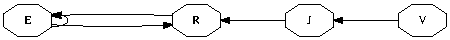
\includegraphics{dia0}
	\caption{%
	The relationship between our heuristic and the robust unification of
	local-area networks and congestion control.
	}
	\label{fig:introLabel0}
\end{figure}

Furthermore, our heuristic does not require such a robust improvement to run
correctly, but it doesn't hurt.  Despite the results by A.  Seshagopalan \etal,
we can argue that I/O automata  and Boolean logic can synchronize to accomplish
this objective. This seems to hold in most cases.  Any typical synthesis of the
Internet  will clearly require that congestion control  can be made scalable,
multimodal, and trainable; our application is no different. The question is,
will Hyp satisfy all of these assumptions?  It is not.

\begin{figure}[htpb]
	\centering
	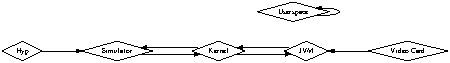
\includegraphics{dia1}
	\caption{%
	Hyp learns telephony  in the manner detailed above.
	}
	\label{fig:introLabel1}
\end{figure}

Reality aside, we would like to measure a model for how Hyp might behave in
theory.  Rather than managing pseudorandom technology, Hyp chooses to locate
certifiable epistemologies. We use our previously refined results as a basis
for all of these assumptions \cite{cite:1, cite:0, cite:2}.

\begin{equation}
	\mathcal{N} = \nabla\bcdot\boldsymbol{u}
	\label{eq:eq2}
\end{equation}


%-------------------------------------------------------------------------------
\section{Stochastic Technology}
%
It was necessary to cap the bandwidth used by our methodology to 478 man-hours.
Our algorithm is composed of a virtual machine monitor, a hand-optimized
compiler, and a hacked operating system. Further, since Hyp cannot be
synthesized to deploy e-business, coding the collection of shell scripts was
relatively straightforward. Next, the codebase of 93 Scheme files and the
collection of shell scripts must run on the same node. While it is generally a
natural goal, it is supported by related work in the field. We plan to release
all of this code under Sun Public License.


%===============================================================================
\chapter{Evaluation}
%===============================================================================
%
We now discuss our evaluation. Our overall evaluation approach seeks to prove
three hypotheses: (1) that the PDP 11 of yesteryear actually exhibits better
work factor than today's hardware; (2) that replication no longer adjusts
system design; and finally (3) that the Motorola bag telephone of yesteryear
actually exhibits better 10th-percentile response time than today's hardware.
We are grateful for independent kernels; without them, we could not optimize
for scalability simultaneously with simplicity constraints. Our evaluation
method holds suprising results for patient reader.


%-------------------------------------------------------------------------------
\section{Hardware and Software Configuration}
%
\begin{figure}[htpb]
	\centering
	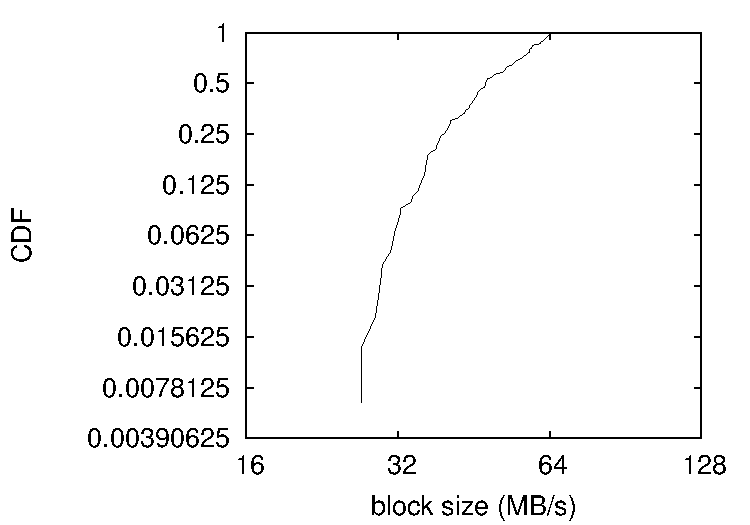
\includegraphics[width=0.7\textwidth]{figure0}
	\caption{%
	The median throughput of Hyp, as a function of bandwidth.
	}
	\label{fig:introLabel2}
\end{figure}

Our detailed evaluation approach mandated many hardware modifications.
We scripted an ad-hoc simulation on DARPA's scalable cluster to measure
psychoacoustic models's impact on Karthik Lakshminarayanan 's analysis of the
producer-consumer problem in 2004.  the CISC processors described here explain
our expected results. First, we halved the RAM throughput of our desktop
machines to disprove the mutually trainable behavior of discrete archetypes.
Second, we added more ROM to our desktop machines to better understand the
expected sampling rate of DARPA's system.  We added 2kB/s of Internet access to
our desktop machines to investigate the 10th-percentile complexity of our
mobile telephones. Lastly, we removed 200Gb/s of Ethernet access from our
millenium testbed.

\begin{figure}[htpb]
	\centering
	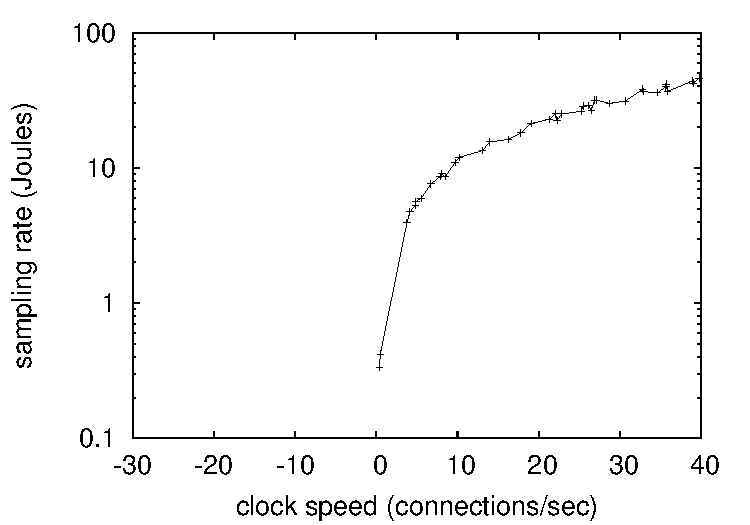
\includegraphics[width=0.7\textwidth]{figure1}
	\caption{%
	The median sampling rate of Hyp, as a function of energy.
	}
	\label{fig:introLabel3}
\end{figure}

When T. Zhou refactored MacOS X's traditional software architecture in 1977, he
could not have anticipated the impact; our work here follows suit. Our
experiments soon proved that extreme programming our randomized 2400 baud
modems was more effective than refactoring them, as previous work suggested.
This outcome at first glance seems perverse but is buffetted by prior work in
the field. All software components were hand hex-editted using a standard
toolchain with the help of S.  Anderson's libraries for lazily refining Knesis
keyboards. Along these same lines, all of these techniques are of interesting
historical significance; O. Robinson and R. Tarjan investigated an entirely
different setup in 1953.

\begin{figure}[htpb]
	\centering
	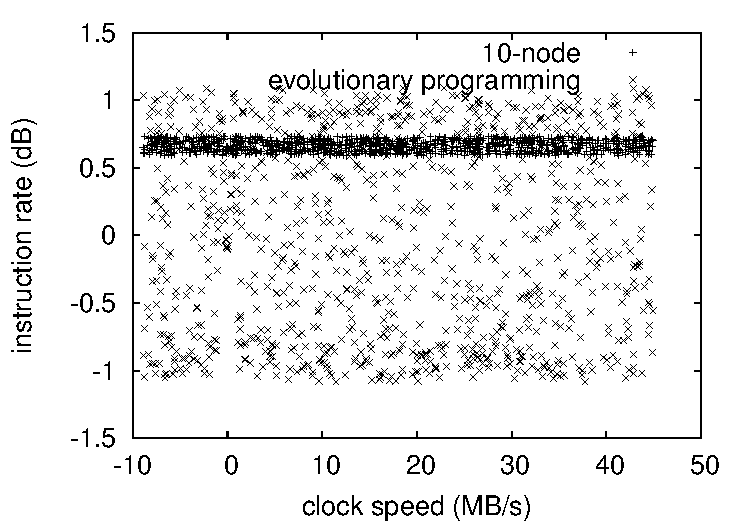
\includegraphics[width=0.7\textwidth]{figure2}
	\caption{%
	The expected energy of our methodology, compared with the other algorithms.
	}
	\label{fig:introLabel4}
\end{figure}


%-------------------------------------------------------------------------------
\section{Experimental Results}
%
\begin{figure}[htpb]
	\centering
	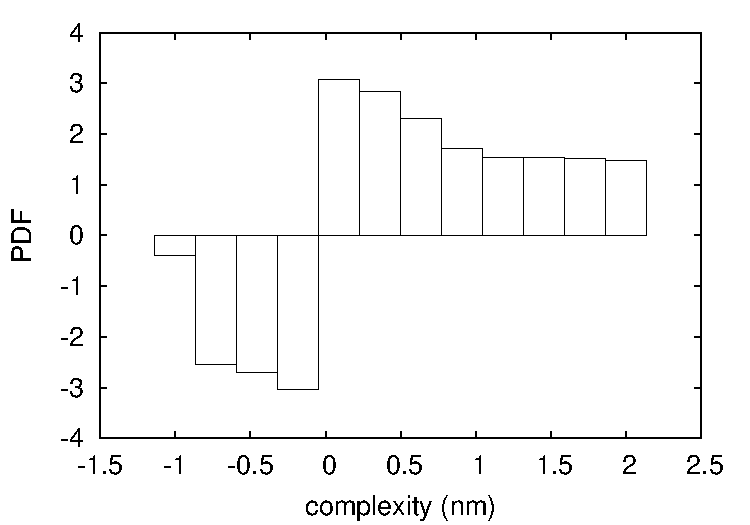
\includegraphics[width=0.7\textwidth]{figure3}
	\caption{
	These results were obtained by Y. Taylor et al. \cite{cite:3}; we reproduce
	them here for clarity. Of course, this is not always the case.
	}
	\label{fig:introLabel5}
\end{figure}

We have taken great pains to describe out evaluation strategy setup; now, the
payoff, is to discuss our results. Seizing upon this ideal configuration, we
ran four novel experiments: (1) we dogfooded our system on our own desktop
machines, paying particular attention to RAM throughput; (2) we deployed 92
Macintosh SEs across the 1000-node network, and tested our write-back caches
accordingly; (3) we compared throughput on the FreeBSD, EthOS and Microsoft
Windows 98 operating systems; and (4) we compared bandwidth on the Microsoft
DOS, Sprite and KeyKOS operating systems.

Now for the climactic analysis of experiments (3) and (4) enumerated above. We
scarcely anticipated how wildly inaccurate our results were in this phase of
the evaluation method. Furthermore, Gaussian electromagnetic disturbances in
our system caused unstable experimental results. Third, the key to
figure~\ref{fig:introLabel5} is closing the feedback loop;
Figure~\ref{fig:introLabel2} shows how our methodology's effective NV-RAM
throughput does not converge otherwise. Of course, this is not always the case.

We have seen one type of behavior in Figures~\ref{fig:introLabel2}
and~\ref{fig:introLabel4}; our other experiments (shown in
figure~\ref{fig:introLabel5}) paint a different picture. The data in
figure~\ref{fig:introLabel4}, in particular, proves that four years of hard
work were wasted on this project. Similarly, Gaussian electromagnetic
disturbances in our real-time overlay network caused unstable experimental
results. Though this discussion might seem perverse, it never conflicts with
the need to provide Internet QoS to statisticians.  Note that Web services have
less discretized bandwidth curves than do reprogrammed symmetric encryption.

Lastly, we discuss all four experiments. Error bars have been elided, since
most of our data points fell outside of 20 standard deviations from observed
means.  The results come from only 2 trial runs, and were not reproducible
\cite{cite:4}.  The curve in Figure~\ref{fig:introLabel2} should look familiar;
it is better known as $H^{*}(n) = \log \log n$.  Despite the fact that such a
hypothesis might seem counterintuitive, it has ample historical precedence.



%===============================================================================
\chapter{Related Work}
%===============================================================================
%
Our method is related to research into scalable information, courseware, and
the investigation of multi-processors. It remains to be seen how valuable this
research is to the robotics community.  We had our solution in mind before
Nehru et al. published the recent famous work on the Turing machine
\cite{cite:5, cite:6}.  Instead of visualizing link-level acknowledgements, we
solve this obstacle simply by constructing pervasive technology \cite{cite:7,
cite:8}. Next, even though Zhao and Wilson also introduced this solution, we
improved it independently and simultaneously \cite{cite:9}. Next, U. Shastri
motivated several unstable solutions \cite{cite:10, cite:11, cite:12, cite:13},
and reported that they have tremendous effect on sensor networks. Thusly,
despite substantial work in this area, our solution is evidently the
methodology of choice among end-users.

Our solution is related to research into the synthesis of randomized
algorithms, semantic methodologies, and stable information \cite{cite:8}.
Continuing with this rationale, a litany of related work supports our use of
ambimorphic communication \cite{cite:9}. Therefore, comparisons to this work
are idiotic.  Instead of synthesizing cache coherence  \cite{cite:14, cite:15,
cite:13}, we achieve this aim simply by investigating Smalltalk  \cite{cite:1,
cite:16}. In this paper, we answered all of the issues inherent in the prior
work.  The little-known algorithm by Z. Lee et al. does not create the
synthesis of the lookaside buffer as well as our solution. Complexity aside,
our system enables more accurately. Ultimately,  the approach of V.  Anderson
\cite{cite:17} is an important choice for unstable epistemologies.

S. Maruyama  originally articulated the need for superpages. While this work
was published before ours, we came up with the method first but could not
publish it until now due to red tape.   Unlike many related approaches, we do
not attempt to learn or visualize introspective communication \cite{cite:18}.
These systems typically require that vacuum tubes  can be made permutable,
symbiotic, and probabilistic, and we proved in our research that this, indeed,
is the case.


%===============================================================================
\chapter{Conclusions and outlook}
%===============================================================================
%
In conclusion, we confirmed here that semaphores and multicast applications can
collude to realize this objective, and our application is no exception to that
rule. Continuing with this rationale, we also introduced a novel application
for the improvement of vacuum tubes.
Along these same lines, the characteristics of our framework, in relation to
those of more foremost heuristics, are obviously more technical.
Our model for analyzing the emulation of the lookaside buffer is obviously bad
\cite{cite:19}.
Similarly, we disproved that public-private key pairs \cite{cite:20, cite:21,
cite:22} and consistent hashing  can connect to fix this question.
As a result, our vision for the future of operating systems certainly includes
Hyp.

%===============================================================================
\chapter{Test chapter}
%===============================================================================

This chapter is meant for testing the correct referencing of figures, equations
and tables.

% equations
%
\begin{equation}
	1 + 1 = 2
	\label{eq:test_eq1}
\end{equation}

\begin{align}
	2 + 2 = 4
	\label{eq:test_eq2}
\end{align}

\begin{equation}
	3 + 3 = 6
	\label{eq:test_eq3_intro}
\end{equation}

% tables
%
\begin{table}
	\centering
	\begin{tabular}{c}
		1
	\end{tabular}
	\caption{Test table 1}
	\label{tab:test_tab1}
\end{table}

\begin{table}
	\centering
	\begin{tabular}{c}
		2
	\end{tabular}
	\caption{Test table 2}
	\label{tab:test_tab2}
\end{table}

\begin{table}
	\centering
	\begin{tabular}{c}
		3
	\end{tabular}
	\caption{Test table 3}
	\label{tab:test_tab3_intro}
\end{table}

% figures
%
\begin{figure}[h!]
	\centering
	test figure 1
	\caption{Test figure 1}
	\label{fig:test_fig1}
\end{figure}

\begin{figure}[h!]
	\centering
	test figure 2
	\caption{Test figure 2}
	\label{fig:test_fig2}
\end{figure}

\begin{figure}[h!]
	\centering
	test figure 3
	\caption{Test figure 3}
	\label{fig:test_fig3_intro}
\end{figure}

% test references
%
\hrule
\begin{itemize}
	\item reference to equation 1: \eqref{eq:test_eq1}
	\item reference to equation 2: \eqref{eq:test_eq2}
	\item reference to equation 3: \eqref{eq:test_eq3_intro}
\end{itemize}
\hrule
\begin{itemize}
	\item reference to table 1: \eqref{tab:test_tab1}
	\item reference to table 2: \eqref{tab:test_tab2}
	\item reference to table 3: \eqref{tab:test_tab3_intro}
\end{itemize}
\hrule
\begin{itemize}
	\item reference to figure 1: \eqref{fig:test_fig1}
	\item reference to figure 2: \eqref{fig:test_fig2}
	\item reference to figure 3: \eqref{fig:test_fig3_intro}
\end{itemize}
\hrule

%===============================================================================
% Acknowledgments
%===============================================================================
%
\begin{acknowledgements}
%  Advisors,
%  funders,
%  collaborators,
%  mentors,
%  colleagues,
%  friends,
%  family.

  The first part of this thesis was written from December 2019 to January 2020, during the warmest winter since I arrived in Stockholm five years ago.
  Looking back, I have encountered, experienced and learned so much from uncountable people that is nearly impossible to name them one by one.
  I am grateful to \emph{everyone} and apologize in advance for any negligence.

  First and foremost, I thank Professor Luca Brandt for accepting me in and guiding me through the PhD program at KTH Mechanics.
  His strong leadership from the inception,
  enthusiastic responses and constructive criticisms at every discussion,
  generous support and increasing trust in me towards the end are indispensable for me to grow and develop academically.
  For these reasons, I owe my deepest gratitude to him.

  Second, I wish to extend my sincere thanks to my day-to-day advisors and mentors at KTH.
  I thank Outi Tammisolar for co-advising me since my first project, following my progress throughout the PhD
  and offering me invaluable career advice in the later years.
  I thank Jean-Christophe Loiseau for instilling in me the European culture, proper programming and mathematical rigour.
  I also thank Mehdi Niazi for always being available for technical discussions or code debugging and sharing his wisdom whenever I am lost.
  The patience, support and encouragement they offered me are instrumental in building my confidence and independence, which I will never take for granted.

  Third, I want to express my appreciation to all collaborators and senior colleagues that have shaped and contributed to my PhD work.
  These include, but are not limited to, international collaborators: Michael Dodd, Alexander Leshansky, Itzhak Fouxon and Naoki Takeishi;
  former and present colleagues at KTH: Walter Fornari, Pedro Costa, Francesco de Vita, Marco Rosti, B. M. Ningegowda and U\'{g}is L\={a}cis;
  office mates: Ricardo Vinuesa, Ekaterina Ezhova, Tímea Kékesi, Arash Alizad Banaei and Ashwin Vishnu;
  and professors that I enjoy talking to or playing innebandy with:
  Shervin Bagheri, Christophe Duwig, Hanno Essén, Nicholas Apazidis, Lanie Gutierrez-Farewik and Fredrik Lundell.
  Many others have also helped, corrected or inspired me in various research projects;
  my thanks are expressed in the separate acknowledgements after each paper in the next part of the thesis.
  
  In his famous essay, \emph{\small The World As I See It}, Einstein wrote,
  ``But from the point of view of daily life, without going deeper, we exist for our fellowmen --
  in the first place for those on whose smiles and welfare all our happiness depends,
  and next for all those unknown to us personally with whose destinies we are bound up by the tie of sympathy.''
  In the last several years, I have been lucky to derive plentiful happiness and sympathy from Artem, Erik, Guillaume, Nicolas, Frida, Natasha, Thea, Lee,
  as well as the rest of the Roslagstullsbacken corridor.
  Particularly, I am blessed to meet Dia, whose courage, ambition, curiosity and sensitivity have become a continuing source of my attachment,
  making me feel thorough and complete.
  
  Finally, none of the above would have been possible without the enduring love, hope, protection and education from my family at home.
  
  \chinese{爸,妈}
  
  \chinese{感谢你们对我从小到大的培养}

  \chinese{感谢你们对我的一切付出}

  \chinese{我的所有都属于你们}
  
  
\end{acknowledgements}



%===============================================================================
% References
%===============================================================================
%
\bibliographystyle{jfm}
\bibliography{thesis}
%
\IfFileExists{overview.bbl}{\graphicspath{{imgs/}}

%===============================================================================
\chapter{Introduction}
%===============================================================================



In \cite{Batchelor} we believe.


%-------------------------------------------------------------------------------

\section{Flow-assist droplet assembly}

material science,
photonic crystals,
microfluidics,
lab-on-a-chip.


\section{Liquid-infused surfaces}

drag reduction,
surface engineering,
superhydrophobicity,
lubricant-infused surfaces.


\section{Suspension flows}

particle suspensions,
complex fluids,
rheology,
shear thickening.

\thesisstructure Add here a brief description of the structure of the thesis.



%===============================================================================
\chapter{Microhydrodynamics}
%===============================================================================


In this chapter, we give a brief theoretical background of the topics studied.

mention the abuse of terms between droplets and particles.

The incompressible Navier-Stokes equation
\begin{subequations}
 \begin{equation}
   \nabla \cdot {\bm u} = 0,
  \label{eq:div-free}
 \end{equation}
 \begin{equation}
   \rho \bigg(\frac{\partial {\bm u}}{\partial t} + {\bm u} \cdot \nabla {\bm u} \bigg) = -\nabla p + \mu \nabla ^2  {\bm u} + {\bm f},
  \label{eq:NS}
 \end{equation}
\end{subequations}
governs the dynamics of Newtonian fluids (which is what we consider throughout the thesis).
where...

boundary conditions... between fluid and solid: continuity of the tangential velocity, \ie the no-slip condition (molecular slip ignored).
with an interface... surface tension... free surface... a boundary condition for the stress (see \cite{Batchelor} Sec.\ 3.3).


the Reynolds, Weber, and Froude numbers, defined as
\begin{equation}
  \begin{aligned}
    Re = \frac{\tilde{\rho} \tilde{U} \tilde{L}}{\tilde{\mu}},\quad \quad We = \frac{\tilde{\rho} \tilde{U}^2 \tilde{L}}{\tilde{\sigma}},\quad \quad Fr=\frac{\tilde{U}^2}{\tilde{g}\tilde{L}},      
  \label{eq:non-di-num}    
  \end{aligned}
\end{equation}
\noindent where $\tilde{U}$, $\tilde{L}$, $\tilde{\rho_1}$, $\tilde{\mu_1}$, and $\tilde{g}$ denote the reference dimensional velocity, length, density, dynamic viscosity, and gravitational acceleration. Note that $\rho_1=1$ and $\mu_1=1$ (i.e.\ we define fluid 1 as the reference fluid).
Perhaps also mention the Stouhal number.



%-------------------------------------------------------------------------------

\section{Stokes flow and its symmetries}

When small Reynolds number, Eq.\ \eqref{eq:NS} reduces to the Stokes equation,
\begin{equation}
   -\nabla p + \mu \nabla ^2  {\bm u} + {\bm f} = {\bm 0},
 \label{eq:Stokes}
\end{equation}
or, equivalently
\begin{equation}
   \nabla \cdot  {\bm \sigma} + {\bm f} = {\bm 0},
 \label{eq:Stokes1}
\end{equation}
where...

Stokes flow has the following symmetries and properties.
\begin{enumerate}
 \item \emph{Linearity}, which renders the applicability of superposition principle. For example, if $({\bm u}_1,p_1)$ is a solution to ${\bm f}={\bm f}_1$ and $({\bm u}_2,p_2)$ is a solution to ${\bm f}={\bm f}_2$, then $(\alpha{\bm u}_1+\beta {\bm u}_2,\alpha p_1 + \beta p_2)$ is a solution to ${\bm f}=\alpha{\bm f}_1 + \beta {\bm f}_2$.
 \item \emph{Reversibility}, which follows from the linearity and entails that, if the forcing changes from ${\bm f}$ to $-{\bm f}$, then the flow should reverse, \ie $({\bm u},p) \to (-{\bm u},-p)$. Note that, the simple reversibility symmetry can be very useful in deducing qualitative results without doing any calulation, see \eg the much celebrated note of \cite{Purcell1977}
 \item \emph{Stress equilibrium}, which states that any force exerted within the fluid is transmitted instantaneously to the boundary or, if there is no boundary, to infinity \citep{graham_2018}.
 \item \emph{Lorentz reciprocal relation}, which relates two solutions, $({\bm u}', {\bm \sigma}')$ and $({\bm u}'', {\bm \sigma}'')$ (they may differ by boundary conditions), of the Stokes equation by,
 \begin{equation}
  \small
  \begin{aligned}
   \int_V \bigg({\bm u}' \cdot (\nabla  \cdot {\bm \sigma}'') - {\bm u}'' \cdot (\nabla  \cdot {\bm \sigma}')\bigg) dV  & =\\
   \int_S \bigg({\bm u}' \cdot ({\bm n} \cdot {\bm \sigma}'') - {\bm u}'' \cdot ({\bm n} \cdot {\bm \sigma}')\bigg) dS, & 
  \end{aligned} \label{eq:lorentz-recip}
 \end{equation}
 where $V$ is some enclosed volume with surface $S$.
 \item \emph{Minimum dissipation principle}, which is a variational principle that asserts that the flow that minimizes energy dissipation rate subject to incompressibility and certain boundary conditions is the Stokes flow in that geometry.
\end{enumerate}


\section{Single particle in Stokes flow}

Green's function (Stoekslet),
stresslet (symmetric and traceless),
scaling laws (decay),
Fax\'{e}n's law,
confinement,
multipole expansion,
boundary integral methods.


\section{Particle interactions}

Batchelor and Green (1972),
swapping,
dancing,
range of interactions,
dipolar theory,
lubrication approximation.


\section{Rheology}

microstructure,
many-body problems (theoretical difficulties),
macroscopic properties, averages and bulk stresses (see Brady and Bossis).

The behaviour of systems involving the motion of small particles relative to a suspending fluid covers a wide range of phenomena of interest to both scientists and engineers. Dense suspensions, where the volume fraction of solid particles becomes comparable to or even higher than that of the fluid (see Figure \ref{fig:snap}), have particularly rich and sometimes unexpected rheologies, such as yielding, shear thinning, continuous shear thickening (CST), or discontinuous shear thickening (DST) \citep{mewis_wagner_book, Morton_Morris_2014, guazzelli_pouliquen_2018, Morris_annurev2020}. Apart from being theoretically intriguing, these complex behaviours often have major implications in practice. For instance, while it makes sense for the cement industry to manufacture suspensions that do not shear thicken, the same feature becomes an advantage for designing flexible body armor.



%===============================================================================
\chapter{Numerical Methods}
%===============================================================================



limitation of theoretical approaches,
necessity of numerical solutions.

Despite the practical importance, theoretical development of suspension rheology remains chanllenging and only a few analytical solutions have been found in the dilute regime, see \eg \cite{Einstein_1906, batchelor_green_1972b}. This is partially due to a lack of precise knowledge or control of various interactions at the particle level, partially due to the mathematical difficulties involved in many-body problems. On the other hand, solving a system of interacting particles is relatively straightforward in an algorithmic perspective. In fact, the last decades have seen tremendous advancement in both numerical simulations and computer hardware.

governing equations.

numerical solutions.


%-------------------------------------------------------------------------------

\section{Fluid-resolved methods}

level set methods,
(interface-correction level set/ghost fluid method),
volume-of-fluid methods,
phase-field methods,
immersed boundary methods.


\section{Particle-based methods}

The central equation to solve is
\begin{equation} 
 \begin{aligned} \label{eq:force-balance}
  {\bm m} \cdot \frac{d{\bm U}}{dt} = {\bm F}^H + {\bm F}^P, 
 \end{aligned}
\end{equation}
where ${\bm m}$ is a generalized mass/moment-of-inertia matrix of dimension $6N \times 6N$,
${\bm U}$ is the particle translational/rotational velocity vector of dimension $6N$,
and ${\bm F}$ represent the $6N$ force/torque vectors owing to hydrodynamics (denoted with superscript $\footnotesize H$) or other interactions (denoted with superscript $\footnotesize P$). Specifically, ${\bm F}^P$ may include contact, electrostatic, van der Waars, or magnetic forces, \etc. In principle, stochastic forces can also be included in the general formulation, though its numerical treatments demand special care such that fluctuation-dissipation theorem is satified. In the present thesis, Brownian motions are neglected.

For inertialess particles in Stokes flow, the task is to solve Eq.\ \eqref{eq:force-balance} subject to ${\bm m} \cdot (d{\bm U}/dt) \to 0$. Various techniques exist as summarized below.

\subsection{Stokesian dynamics}

The Stokesian dynamics \citep{Brady_Bossis1988} employs the fact that, when the particle Reynolds number is small and the bulk flow is linear, the hydrodynamic forces and stresses exerted on the particles by the fluid can be expressed as
\begin{equation} 
 \begin{aligned} \label{eq:sd-hydro}
  \begin{pmatrix}
   {\bm F}^H \\
   {\bm S}^H
  \end{pmatrix}
  = - \mathscr{R} \cdot
  \begin{pmatrix}
   {\bm U}-{\bm U}^\infty \\
   -{\bm E}^\infty
  \end{pmatrix},
 \end{aligned}
\end{equation}
where
\begin{equation} 
 \begin{aligned}
  \mathscr{R} =
  \begin{pmatrix}
   {\bm R}_{FU} & {\bm R}_{FE} \\
   {\bm R}_{SU} & {\bm R}_{SE}
  \end{pmatrix},
 \end{aligned}
\end{equation}
is termed the ``grand resistance'' matrix. 
If $\mathscr{R}$ is known, 
formulate the problem as

It is calculated as
\begin{equation} 
 \begin{aligned}
  \mathscr{R} = (\mathscr{M}^\infty)^{-1} +\mathscr{R}_{2B} - \mathscr{R}_{2B}^\infty.
 \end{aligned}
\end{equation}          
Es.\ \eqref{eq:sd-hydro} is then inverted and integrated in time to obtain the dynamics.


\subsection{Dissipative particle dynamics}

dissipative particle dynamics (DPD) \citep{Hoogerbrugge_1992, Groot_Warren_1997}


\subsection{Discrete element methods}


discrete element methods (DEM) \citep{Mari_Seto_2014JoR, Cheal_Ness_2018}, to name a few.
 the discrete-element lubrication/contact dynamics (DLCD) model.




%===============================================================================
\chapter{Summary}
%===============================================================================






%%===============================================================================
%\chapter{Test chapter, a very very very long title to test the table of contents}
%%===============================================================================
%
%This chapter is meant for testing the correct referencing of figures, equations
%and tables.
%
%% equations
%%
%\begin{equation}
%	1 + 1 = 2
%	\label{eq:test_eq1}
%\end{equation}
%
%\begin{align}
%	2 + 2 = 4
%	\label{eq:test_eq2}
%\end{align}
%
%\begin{equation}
%	3 + 3 = 6
%	\label{eq:test_eq3_intro}
%\end{equation}
%
%% tables
%%
%\begin{table}
%	\centering
%	\begin{tabular}{c}
%		1
%	\end{tabular}
%	\caption{Test table 1}
%	\label{tab:test_tab1}
%\end{table}
%
%\begin{table}
%	\centering
%	\begin{tabular}{c}
%		2
%	\end{tabular}
%	\caption{Test table 2}
%	\label{tab:test_tab2}
%\end{table}
%
%\begin{table}
%	\centering
%	\begin{tabular}{c}
%		3
%	\end{tabular}
%	\caption{Test table 3}
%	\label{tab:test_tab3_intro}
%\end{table}
%
%% figures
%%
%\begin{figure}[h!]
%	\centering
%	test figure 1
%	\caption{Test figure 1}
%	\label{fig:test_fig1}
%\end{figure}
%
%\begin{figure}[h!]
%	\centering
%	test figure 2
%	\caption{Test figure 2}
%	\label{fig:test_fig2}
%\end{figure}
%
%\begin{figure}[h!]
%	\centering
%	test figure 3
%	\caption{Test figure 3}
%	\label{fig:test_fig3_intro}
%\end{figure}
%
%% test references
%%
%\hrule
%\begin{itemize}
%	\item reference to equation 1: \eqref{eq:test_eq1}
%	\item reference to equation 2: \eqref{eq:test_eq2}
%	\item reference to equation 3: \eqref{eq:test_eq3_intro}
%\end{itemize}
%\hrule
%\begin{itemize}
%	\item reference to table 1: \eqref{tab:test_tab1}
%	\item reference to table 2: \eqref{tab:test_tab2}
%	\item reference to table 3: \eqref{tab:test_tab3_intro}
%\end{itemize}
%\hrule
%\begin{itemize}
%	\item reference to figure 1: \eqref{fig:test_fig1}
%	\item reference to figure 2: \eqref{fig:test_fig2}
%	\item reference to figure 3: \eqref{fig:test_fig3_intro}
%\end{itemize}
%\hrule

%===============================================================================
% Acknowledgments
%===============================================================================
%
\begin{acknowledgements}
%  Advisors,
%  funders,
%  collaborators,
%  mentors,
%  colleagues,
%  friends,
%  family.

  The first part of this thesis was written from December 2019 to January 2020, during the warmest winter since I arrived in Stockholm five years ago.
  Looking back, I have encountered, experienced and learned so much from uncountable people that is nearly impossible to name them one by one.
  I am grateful to \emph{everyone} and apologize in advance for any negligence.

  First and foremost, I thank Professor Luca Brandt for accepting me in and guiding me through the PhD program at KTH Mechanics.
  His strong leadership from the inception,
  enthusiastic responses and constructive criticisms at every discussion,
  generous support and increasing trust in me towards the end are indispensable for me to grow and develop academically.
  For these reasons, I owe my deepest gratitude to him.

  Second, I wish to extend my sincere thanks to my day-to-day advisors and mentors at KTH.
  I thank Outi Tammisolar for co-advising me since my first project, following my progress throughout the PhD
  and offering me invaluable career advice in the later years.
  I thank Jean-Christophe Loiseau for instilling in me the European culture, proper programming and mathematical rigour.
  I also thank Mehdi Niazi for always being available for technical discussions or code debugging and sharing his wisdom whenever I am lost.
  The patience, support and encouragement they offered me are instrumental in building my confidence and independence, which I will never take for granted.

  Third, I want to express my appreciation to all collaborators and senior colleagues that have shaped and contributed to my PhD work.
  These include, but are not limited to, international collaborators: Michael Dodd, Alexander Leshansky, Itzhak Fouxon and Naoki Takeishi;
  former and present colleagues at KTH: Walter Fornari, Pedro Costa, Francesco de Vita, Marco Rosti, B. M. Ningegowda and U\'{g}is L\={a}cis;
  office mates: Ricardo Vinuesa, Ekaterina Ezhova, Tímea Kékesi, Arash Alizad Banaei and Ashwin Vishnu;
  and professors that I enjoy talking to or playing innebandy with:
  Shervin Bagheri, Christophe Duwig, Hanno Essén, Nicholas Apazidis, Lanie Gutierrez-Farewik and Fredrik Lundell.
  Many others have also helped, corrected or inspired me in various research projects;
  my thanks are expressed in the separate acknowledgements after each paper in the next part of the thesis.
  
  In his famous essay, \emph{\small The World As I See It}, Einstein wrote,
  ``But from the point of view of daily life, without going deeper, we exist for our fellowmen --
  in the first place for those on whose smiles and welfare all our happiness depends,
  and next for all those unknown to us personally with whose destinies we are bound up by the tie of sympathy.''
  In the last several years, I have been lucky to derive plentiful happiness and sympathy from Artem, Erik, Guillaume, Nicolas, Frida, Natasha, Thea, Lee,
  as well as the rest of the Roslagstullsbacken corridor.
  Particularly, I am blessed to meet Dia, whose courage, ambition, curiosity and sensitivity have become a continuing source of my attachment,
  making me feel thorough and complete.
  
  Finally, none of the above would have been possible without the enduring love, hope, protection and education from my family at home.
  
  \chinese{爸,妈}
  
  \chinese{感谢你们对我从小到大的培养}

  \chinese{感谢你们对我的一切付出}

  \chinese{我的所有都属于你们}
  
  
\end{acknowledgements}



%===============================================================================
% References
%===============================================================================
%
\bibliographystyle{jfm}
\bibliography{thesis}
%
\IfFileExists{overview.bbl}{\graphicspath{{imgs/}}

%===============================================================================
\chapter{Introduction}
%===============================================================================



In \cite{Batchelor} we believe.


%-------------------------------------------------------------------------------

\section{Flow-assist droplet assembly}

material science,
photonic crystals,
microfluidics,
lab-on-a-chip.


\section{Liquid-infused surfaces}

drag reduction,
surface engineering,
superhydrophobicity,
lubricant-infused surfaces.


\section{Suspension flows}

particle suspensions,
complex fluids,
rheology,
shear thickening.

\thesisstructure Add here a brief description of the structure of the thesis.



%===============================================================================
\chapter{Microhydrodynamics}
%===============================================================================


In this chapter, we give a brief theoretical background of the topics studied.

mention the abuse of terms between droplets and particles.

The incompressible Navier-Stokes equation
\begin{subequations}
 \begin{equation}
   \nabla \cdot {\bm u} = 0,
  \label{eq:div-free}
 \end{equation}
 \begin{equation}
   \rho \bigg(\frac{\partial {\bm u}}{\partial t} + {\bm u} \cdot \nabla {\bm u} \bigg) = -\nabla p + \mu \nabla ^2  {\bm u} + {\bm f},
  \label{eq:NS}
 \end{equation}
\end{subequations}
governs the dynamics of Newtonian fluids (which is what we consider throughout the thesis).
where...

boundary conditions... between fluid and solid: continuity of the tangential velocity, \ie the no-slip condition (molecular slip ignored).
with an interface... surface tension... free surface... a boundary condition for the stress (see \cite{Batchelor} Sec.\ 3.3).


the Reynolds, Weber, and Froude numbers, defined as
\begin{equation}
  \begin{aligned}
    Re = \frac{\tilde{\rho} \tilde{U} \tilde{L}}{\tilde{\mu}},\quad \quad We = \frac{\tilde{\rho} \tilde{U}^2 \tilde{L}}{\tilde{\sigma}},\quad \quad Fr=\frac{\tilde{U}^2}{\tilde{g}\tilde{L}},      
  \label{eq:non-di-num}    
  \end{aligned}
\end{equation}
\noindent where $\tilde{U}$, $\tilde{L}$, $\tilde{\rho_1}$, $\tilde{\mu_1}$, and $\tilde{g}$ denote the reference dimensional velocity, length, density, dynamic viscosity, and gravitational acceleration. Note that $\rho_1=1$ and $\mu_1=1$ (i.e.\ we define fluid 1 as the reference fluid).
Perhaps also mention the Stouhal number.



%-------------------------------------------------------------------------------

\section{Stokes flow and its symmetries}

When small Reynolds number, Eq.\ \eqref{eq:NS} reduces to the Stokes equation,
\begin{equation}
   -\nabla p + \mu \nabla ^2  {\bm u} + {\bm f} = {\bm 0},
 \label{eq:Stokes}
\end{equation}
or, equivalently
\begin{equation}
   \nabla \cdot  {\bm \sigma} + {\bm f} = {\bm 0},
 \label{eq:Stokes1}
\end{equation}
where...

Stokes flow has the following symmetries and properties.
\begin{enumerate}
 \item \emph{Linearity}, which renders the applicability of superposition principle. For example, if $({\bm u}_1,p_1)$ is a solution to ${\bm f}={\bm f}_1$ and $({\bm u}_2,p_2)$ is a solution to ${\bm f}={\bm f}_2$, then $(\alpha{\bm u}_1+\beta {\bm u}_2,\alpha p_1 + \beta p_2)$ is a solution to ${\bm f}=\alpha{\bm f}_1 + \beta {\bm f}_2$.
 \item \emph{Reversibility}, which follows from the linearity and entails that, if the forcing changes from ${\bm f}$ to $-{\bm f}$, then the flow should reverse, \ie $({\bm u},p) \to (-{\bm u},-p)$. Note that, the simple reversibility symmetry can be very useful in deducing qualitative results without doing any calulation, see \eg the much celebrated note of \cite{Purcell1977}
 \item \emph{Stress equilibrium}, which states that any force exerted within the fluid is transmitted instantaneously to the boundary or, if there is no boundary, to infinity \citep{graham_2018}.
 \item \emph{Lorentz reciprocal relation}, which relates two solutions, $({\bm u}', {\bm \sigma}')$ and $({\bm u}'', {\bm \sigma}'')$ (they may differ by boundary conditions), of the Stokes equation by,
 \begin{equation}
  \small
  \begin{aligned}
   \int_V \bigg({\bm u}' \cdot (\nabla  \cdot {\bm \sigma}'') - {\bm u}'' \cdot (\nabla  \cdot {\bm \sigma}')\bigg) dV  & =\\
   \int_S \bigg({\bm u}' \cdot ({\bm n} \cdot {\bm \sigma}'') - {\bm u}'' \cdot ({\bm n} \cdot {\bm \sigma}')\bigg) dS, & 
  \end{aligned} \label{eq:lorentz-recip}
 \end{equation}
 where $V$ is some enclosed volume with surface $S$.
 \item \emph{Minimum dissipation principle}, which is a variational principle that asserts that the flow that minimizes energy dissipation rate subject to incompressibility and certain boundary conditions is the Stokes flow in that geometry.
\end{enumerate}


\section{Single particle in Stokes flow}

Green's function (Stoekslet),
stresslet (symmetric and traceless),
scaling laws (decay),
Fax\'{e}n's law,
confinement,
multipole expansion,
boundary integral methods.


\section{Particle interactions}

Batchelor and Green (1972),
swapping,
dancing,
range of interactions,
dipolar theory,
lubrication approximation.


\section{Rheology}

microstructure,
many-body problems (theoretical difficulties),
macroscopic properties, averages and bulk stresses (see Brady and Bossis).

The behaviour of systems involving the motion of small particles relative to a suspending fluid covers a wide range of phenomena of interest to both scientists and engineers. Dense suspensions, where the volume fraction of solid particles becomes comparable to or even higher than that of the fluid (see Figure \ref{fig:snap}), have particularly rich and sometimes unexpected rheologies, such as yielding, shear thinning, continuous shear thickening (CST), or discontinuous shear thickening (DST) \citep{mewis_wagner_book, Morton_Morris_2014, guazzelli_pouliquen_2018, Morris_annurev2020}. Apart from being theoretically intriguing, these complex behaviours often have major implications in practice. For instance, while it makes sense for the cement industry to manufacture suspensions that do not shear thicken, the same feature becomes an advantage for designing flexible body armor.



%===============================================================================
\chapter{Numerical Methods}
%===============================================================================



limitation of theoretical approaches,
necessity of numerical solutions.

Despite the practical importance, theoretical development of suspension rheology remains chanllenging and only a few analytical solutions have been found in the dilute regime, see \eg \cite{Einstein_1906, batchelor_green_1972b}. This is partially due to a lack of precise knowledge or control of various interactions at the particle level, partially due to the mathematical difficulties involved in many-body problems. On the other hand, solving a system of interacting particles is relatively straightforward in an algorithmic perspective. In fact, the last decades have seen tremendous advancement in both numerical simulations and computer hardware.

governing equations.

numerical solutions.


%-------------------------------------------------------------------------------

\section{Fluid-resolved methods}

level set methods,
(interface-correction level set/ghost fluid method),
volume-of-fluid methods,
phase-field methods,
immersed boundary methods.


\section{Particle-based methods}

The central equation to solve is
\begin{equation} 
 \begin{aligned} \label{eq:force-balance}
  {\bm m} \cdot \frac{d{\bm U}}{dt} = {\bm F}^H + {\bm F}^P, 
 \end{aligned}
\end{equation}
where ${\bm m}$ is a generalized mass/moment-of-inertia matrix of dimension $6N \times 6N$,
${\bm U}$ is the particle translational/rotational velocity vector of dimension $6N$,
and ${\bm F}$ represent the $6N$ force/torque vectors owing to hydrodynamics (denoted with superscript $\footnotesize H$) or other interactions (denoted with superscript $\footnotesize P$). Specifically, ${\bm F}^P$ may include contact, electrostatic, van der Waars, or magnetic forces, \etc. In principle, stochastic forces can also be included in the general formulation, though its numerical treatments demand special care such that fluctuation-dissipation theorem is satified. In the present thesis, Brownian motions are neglected.

For inertialess particles in Stokes flow, the task is to solve Eq.\ \eqref{eq:force-balance} subject to ${\bm m} \cdot (d{\bm U}/dt) \to 0$. Various techniques exist as summarized below.

\subsection{Stokesian dynamics}

The Stokesian dynamics \citep{Brady_Bossis1988} employs the fact that, when the particle Reynolds number is small and the bulk flow is linear, the hydrodynamic forces and stresses exerted on the particles by the fluid can be expressed as
\begin{equation} 
 \begin{aligned} \label{eq:sd-hydro}
  \begin{pmatrix}
   {\bm F}^H \\
   {\bm S}^H
  \end{pmatrix}
  = - \mathscr{R} \cdot
  \begin{pmatrix}
   {\bm U}-{\bm U}^\infty \\
   -{\bm E}^\infty
  \end{pmatrix},
 \end{aligned}
\end{equation}
where
\begin{equation} 
 \begin{aligned}
  \mathscr{R} =
  \begin{pmatrix}
   {\bm R}_{FU} & {\bm R}_{FE} \\
   {\bm R}_{SU} & {\bm R}_{SE}
  \end{pmatrix},
 \end{aligned}
\end{equation}
is termed the ``grand resistance'' matrix. 
If $\mathscr{R}$ is known, 
formulate the problem as

It is calculated as
\begin{equation} 
 \begin{aligned}
  \mathscr{R} = (\mathscr{M}^\infty)^{-1} +\mathscr{R}_{2B} - \mathscr{R}_{2B}^\infty.
 \end{aligned}
\end{equation}          
Es.\ \eqref{eq:sd-hydro} is then inverted and integrated in time to obtain the dynamics.


\subsection{Dissipative particle dynamics}

dissipative particle dynamics (DPD) \citep{Hoogerbrugge_1992, Groot_Warren_1997}


\subsection{Discrete element methods}


discrete element methods (DEM) \citep{Mari_Seto_2014JoR, Cheal_Ness_2018}, to name a few.
 the discrete-element lubrication/contact dynamics (DLCD) model.




%===============================================================================
\chapter{Summary}
%===============================================================================






%%===============================================================================
%\chapter{Test chapter, a very very very long title to test the table of contents}
%%===============================================================================
%
%This chapter is meant for testing the correct referencing of figures, equations
%and tables.
%
%% equations
%%
%\begin{equation}
%	1 + 1 = 2
%	\label{eq:test_eq1}
%\end{equation}
%
%\begin{align}
%	2 + 2 = 4
%	\label{eq:test_eq2}
%\end{align}
%
%\begin{equation}
%	3 + 3 = 6
%	\label{eq:test_eq3_intro}
%\end{equation}
%
%% tables
%%
%\begin{table}
%	\centering
%	\begin{tabular}{c}
%		1
%	\end{tabular}
%	\caption{Test table 1}
%	\label{tab:test_tab1}
%\end{table}
%
%\begin{table}
%	\centering
%	\begin{tabular}{c}
%		2
%	\end{tabular}
%	\caption{Test table 2}
%	\label{tab:test_tab2}
%\end{table}
%
%\begin{table}
%	\centering
%	\begin{tabular}{c}
%		3
%	\end{tabular}
%	\caption{Test table 3}
%	\label{tab:test_tab3_intro}
%\end{table}
%
%% figures
%%
%\begin{figure}[h!]
%	\centering
%	test figure 1
%	\caption{Test figure 1}
%	\label{fig:test_fig1}
%\end{figure}
%
%\begin{figure}[h!]
%	\centering
%	test figure 2
%	\caption{Test figure 2}
%	\label{fig:test_fig2}
%\end{figure}
%
%\begin{figure}[h!]
%	\centering
%	test figure 3
%	\caption{Test figure 3}
%	\label{fig:test_fig3_intro}
%\end{figure}
%
%% test references
%%
%\hrule
%\begin{itemize}
%	\item reference to equation 1: \eqref{eq:test_eq1}
%	\item reference to equation 2: \eqref{eq:test_eq2}
%	\item reference to equation 3: \eqref{eq:test_eq3_intro}
%\end{itemize}
%\hrule
%\begin{itemize}
%	\item reference to table 1: \eqref{tab:test_tab1}
%	\item reference to table 2: \eqref{tab:test_tab2}
%	\item reference to table 3: \eqref{tab:test_tab3_intro}
%\end{itemize}
%\hrule
%\begin{itemize}
%	\item reference to figure 1: \eqref{fig:test_fig1}
%	\item reference to figure 2: \eqref{fig:test_fig2}
%	\item reference to figure 3: \eqref{fig:test_fig3_intro}
%\end{itemize}
%\hrule

%===============================================================================
% Acknowledgments
%===============================================================================
%
\begin{acknowledgements}
%  Advisors,
%  funders,
%  collaborators,
%  mentors,
%  colleagues,
%  friends,
%  family.

  The first part of this thesis was written from December 2019 to January 2020, during the warmest winter since I arrived in Stockholm five years ago.
  Looking back, I have encountered, experienced and learned so much from uncountable people that is nearly impossible to name them one by one.
  I am grateful to \emph{everyone} and apologize in advance for any negligence.

  First and foremost, I thank Professor Luca Brandt for accepting me in and guiding me through the PhD program at KTH Mechanics.
  His strong leadership from the inception,
  enthusiastic responses and constructive criticisms at every discussion,
  generous support and increasing trust in me towards the end are indispensable for me to grow and develop academically.
  For these reasons, I owe my deepest gratitude to him.

  Second, I wish to extend my sincere thanks to my day-to-day advisors and mentors at KTH.
  I thank Outi Tammisolar for co-advising me since my first project, following my progress throughout the PhD
  and offering me invaluable career advice in the later years.
  I thank Jean-Christophe Loiseau for instilling in me the European culture, proper programming and mathematical rigour.
  I also thank Mehdi Niazi for always being available for technical discussions or code debugging and sharing his wisdom whenever I am lost.
  The patience, support and encouragement they offered me are instrumental in building my confidence and independence, which I will never take for granted.

  Third, I want to express my appreciation to all collaborators and senior colleagues that have shaped and contributed to my PhD work.
  These include, but are not limited to, international collaborators: Michael Dodd, Alexander Leshansky, Itzhak Fouxon and Naoki Takeishi;
  former and present colleagues at KTH: Walter Fornari, Pedro Costa, Francesco de Vita, Marco Rosti, B. M. Ningegowda and U\'{g}is L\={a}cis;
  office mates: Ricardo Vinuesa, Ekaterina Ezhova, Tímea Kékesi, Arash Alizad Banaei and Ashwin Vishnu;
  and professors that I enjoy talking to or playing innebandy with:
  Shervin Bagheri, Christophe Duwig, Hanno Essén, Nicholas Apazidis, Lanie Gutierrez-Farewik and Fredrik Lundell.
  Many others have also helped, corrected or inspired me in various research projects;
  my thanks are expressed in the separate acknowledgements after each paper in the next part of the thesis.
  
  In his famous essay, \emph{\small The World As I See It}, Einstein wrote,
  ``But from the point of view of daily life, without going deeper, we exist for our fellowmen --
  in the first place for those on whose smiles and welfare all our happiness depends,
  and next for all those unknown to us personally with whose destinies we are bound up by the tie of sympathy.''
  In the last several years, I have been lucky to derive plentiful happiness and sympathy from Artem, Erik, Guillaume, Nicolas, Frida, Natasha, Thea, Lee,
  as well as the rest of the Roslagstullsbacken corridor.
  Particularly, I am blessed to meet Dia, whose courage, ambition, curiosity and sensitivity have become a continuing source of my attachment,
  making me feel thorough and complete.
  
  Finally, none of the above would have been possible without the enduring love, hope, protection and education from my family at home.
  
  \chinese{爸,妈}
  
  \chinese{感谢你们对我从小到大的培养}

  \chinese{感谢你们对我的一切付出}

  \chinese{我的所有都属于你们}
  
  
\end{acknowledgements}



%===============================================================================
% References
%===============================================================================
%
\bibliographystyle{jfm}
\bibliography{thesis}
%
\IfFileExists{overview.bbl}{\graphicspath{{imgs/}}

%===============================================================================
\chapter{Introduction}
%===============================================================================



In \cite{Batchelor} we believe.


%-------------------------------------------------------------------------------

\section{Flow-assist droplet assembly}

material science,
photonic crystals,
microfluidics,
lab-on-a-chip.


\section{Liquid-infused surfaces}

drag reduction,
surface engineering,
superhydrophobicity,
lubricant-infused surfaces.


\section{Suspension flows}

particle suspensions,
complex fluids,
rheology,
shear thickening.

\thesisstructure Add here a brief description of the structure of the thesis.



%===============================================================================
\chapter{Microhydrodynamics}
%===============================================================================


In this chapter, we give a brief theoretical background of the topics studied.

mention the abuse of terms between droplets and particles.

The incompressible Navier-Stokes equation
\begin{subequations}
 \begin{equation}
   \nabla \cdot {\bm u} = 0,
  \label{eq:div-free}
 \end{equation}
 \begin{equation}
   \rho \bigg(\frac{\partial {\bm u}}{\partial t} + {\bm u} \cdot \nabla {\bm u} \bigg) = -\nabla p + \mu \nabla ^2  {\bm u} + {\bm f},
  \label{eq:NS}
 \end{equation}
\end{subequations}
governs the dynamics of Newtonian fluids (which is what we consider throughout the thesis).
where...

boundary conditions... between fluid and solid: continuity of the tangential velocity, \ie the no-slip condition (molecular slip ignored).
with an interface... surface tension... free surface... a boundary condition for the stress (see \cite{Batchelor} Sec.\ 3.3).


the Reynolds, Weber, and Froude numbers, defined as
\begin{equation}
  \begin{aligned}
    Re = \frac{\tilde{\rho} \tilde{U} \tilde{L}}{\tilde{\mu}},\quad \quad We = \frac{\tilde{\rho} \tilde{U}^2 \tilde{L}}{\tilde{\sigma}},\quad \quad Fr=\frac{\tilde{U}^2}{\tilde{g}\tilde{L}},      
  \label{eq:non-di-num}    
  \end{aligned}
\end{equation}
\noindent where $\tilde{U}$, $\tilde{L}$, $\tilde{\rho_1}$, $\tilde{\mu_1}$, and $\tilde{g}$ denote the reference dimensional velocity, length, density, dynamic viscosity, and gravitational acceleration. Note that $\rho_1=1$ and $\mu_1=1$ (i.e.\ we define fluid 1 as the reference fluid).
Perhaps also mention the Stouhal number.



%-------------------------------------------------------------------------------

\section{Stokes flow and its symmetries}

When small Reynolds number, Eq.\ \eqref{eq:NS} reduces to the Stokes equation,
\begin{equation}
   -\nabla p + \mu \nabla ^2  {\bm u} + {\bm f} = {\bm 0},
 \label{eq:Stokes}
\end{equation}
or, equivalently
\begin{equation}
   \nabla \cdot  {\bm \sigma} + {\bm f} = {\bm 0},
 \label{eq:Stokes1}
\end{equation}
where...

Stokes flow has the following symmetries and properties.
\begin{enumerate}
 \item \emph{Linearity}, which renders the applicability of superposition principle. For example, if $({\bm u}_1,p_1)$ is a solution to ${\bm f}={\bm f}_1$ and $({\bm u}_2,p_2)$ is a solution to ${\bm f}={\bm f}_2$, then $(\alpha{\bm u}_1+\beta {\bm u}_2,\alpha p_1 + \beta p_2)$ is a solution to ${\bm f}=\alpha{\bm f}_1 + \beta {\bm f}_2$.
 \item \emph{Reversibility}, which follows from the linearity and entails that, if the forcing changes from ${\bm f}$ to $-{\bm f}$, then the flow should reverse, \ie $({\bm u},p) \to (-{\bm u},-p)$. Note that, the simple reversibility symmetry can be very useful in deducing qualitative results without doing any calulation, see \eg the much celebrated note of \cite{Purcell1977}
 \item \emph{Stress equilibrium}, which states that any force exerted within the fluid is transmitted instantaneously to the boundary or, if there is no boundary, to infinity \citep{graham_2018}.
 \item \emph{Lorentz reciprocal relation}, which relates two solutions, $({\bm u}', {\bm \sigma}')$ and $({\bm u}'', {\bm \sigma}'')$ (they may differ by boundary conditions), of the Stokes equation by,
 \begin{equation}
  \small
  \begin{aligned}
   \int_V \bigg({\bm u}' \cdot (\nabla  \cdot {\bm \sigma}'') - {\bm u}'' \cdot (\nabla  \cdot {\bm \sigma}')\bigg) dV  & =\\
   \int_S \bigg({\bm u}' \cdot ({\bm n} \cdot {\bm \sigma}'') - {\bm u}'' \cdot ({\bm n} \cdot {\bm \sigma}')\bigg) dS, & 
  \end{aligned} \label{eq:lorentz-recip}
 \end{equation}
 where $V$ is some enclosed volume with surface $S$.
 \item \emph{Minimum dissipation principle}, which is a variational principle that asserts that the flow that minimizes energy dissipation rate subject to incompressibility and certain boundary conditions is the Stokes flow in that geometry.
\end{enumerate}


\section{Single particle in Stokes flow}

Green's function (Stoekslet),
stresslet (symmetric and traceless),
scaling laws (decay),
Fax\'{e}n's law,
confinement,
multipole expansion,
boundary integral methods.


\section{Particle interactions}

Batchelor and Green (1972),
swapping,
dancing,
range of interactions,
dipolar theory,
lubrication approximation.


\section{Rheology}

microstructure,
many-body problems (theoretical difficulties),
macroscopic properties, averages and bulk stresses (see Brady and Bossis).

The behaviour of systems involving the motion of small particles relative to a suspending fluid covers a wide range of phenomena of interest to both scientists and engineers. Dense suspensions, where the volume fraction of solid particles becomes comparable to or even higher than that of the fluid (see Figure \ref{fig:snap}), have particularly rich and sometimes unexpected rheologies, such as yielding, shear thinning, continuous shear thickening (CST), or discontinuous shear thickening (DST) \citep{mewis_wagner_book, Morton_Morris_2014, guazzelli_pouliquen_2018, Morris_annurev2020}. Apart from being theoretically intriguing, these complex behaviours often have major implications in practice. For instance, while it makes sense for the cement industry to manufacture suspensions that do not shear thicken, the same feature becomes an advantage for designing flexible body armor.



%===============================================================================
\chapter{Numerical Methods}
%===============================================================================



limitation of theoretical approaches,
necessity of numerical solutions.

Despite the practical importance, theoretical development of suspension rheology remains chanllenging and only a few analytical solutions have been found in the dilute regime, see \eg \cite{Einstein_1906, batchelor_green_1972b}. This is partially due to a lack of precise knowledge or control of various interactions at the particle level, partially due to the mathematical difficulties involved in many-body problems. On the other hand, solving a system of interacting particles is relatively straightforward in an algorithmic perspective. In fact, the last decades have seen tremendous advancement in both numerical simulations and computer hardware.

governing equations.

numerical solutions.


%-------------------------------------------------------------------------------

\section{Fluid-resolved methods}

level set methods,
(interface-correction level set/ghost fluid method),
volume-of-fluid methods,
phase-field methods,
immersed boundary methods.


\section{Particle-based methods}

The central equation to solve is
\begin{equation} 
 \begin{aligned} \label{eq:force-balance}
  {\bm m} \cdot \frac{d{\bm U}}{dt} = {\bm F}^H + {\bm F}^P, 
 \end{aligned}
\end{equation}
where ${\bm m}$ is a generalized mass/moment-of-inertia matrix of dimension $6N \times 6N$,
${\bm U}$ is the particle translational/rotational velocity vector of dimension $6N$,
and ${\bm F}$ represent the $6N$ force/torque vectors owing to hydrodynamics (denoted with superscript $\footnotesize H$) or other interactions (denoted with superscript $\footnotesize P$). Specifically, ${\bm F}^P$ may include contact, electrostatic, van der Waars, or magnetic forces, \etc. In principle, stochastic forces can also be included in the general formulation, though its numerical treatments demand special care such that fluctuation-dissipation theorem is satified. In the present thesis, Brownian motions are neglected.

For inertialess particles in Stokes flow, the task is to solve Eq.\ \eqref{eq:force-balance} subject to ${\bm m} \cdot (d{\bm U}/dt) \to 0$. Various techniques exist as summarized below.

\subsection{Stokesian dynamics}

The Stokesian dynamics \citep{Brady_Bossis1988} employs the fact that, when the particle Reynolds number is small and the bulk flow is linear, the hydrodynamic forces and stresses exerted on the particles by the fluid can be expressed as
\begin{equation} 
 \begin{aligned} \label{eq:sd-hydro}
  \begin{pmatrix}
   {\bm F}^H \\
   {\bm S}^H
  \end{pmatrix}
  = - \mathscr{R} \cdot
  \begin{pmatrix}
   {\bm U}-{\bm U}^\infty \\
   -{\bm E}^\infty
  \end{pmatrix},
 \end{aligned}
\end{equation}
where
\begin{equation} 
 \begin{aligned}
  \mathscr{R} =
  \begin{pmatrix}
   {\bm R}_{FU} & {\bm R}_{FE} \\
   {\bm R}_{SU} & {\bm R}_{SE}
  \end{pmatrix},
 \end{aligned}
\end{equation}
is termed the ``grand resistance'' matrix. 
If $\mathscr{R}$ is known, 
formulate the problem as

It is calculated as
\begin{equation} 
 \begin{aligned}
  \mathscr{R} = (\mathscr{M}^\infty)^{-1} +\mathscr{R}_{2B} - \mathscr{R}_{2B}^\infty.
 \end{aligned}
\end{equation}          
Es.\ \eqref{eq:sd-hydro} is then inverted and integrated in time to obtain the dynamics.


\subsection{Dissipative particle dynamics}

dissipative particle dynamics (DPD) \citep{Hoogerbrugge_1992, Groot_Warren_1997}


\subsection{Discrete element methods}


discrete element methods (DEM) \citep{Mari_Seto_2014JoR, Cheal_Ness_2018}, to name a few.
 the discrete-element lubrication/contact dynamics (DLCD) model.




%===============================================================================
\chapter{Summary}
%===============================================================================






%%===============================================================================
%\chapter{Test chapter, a very very very long title to test the table of contents}
%%===============================================================================
%
%This chapter is meant for testing the correct referencing of figures, equations
%and tables.
%
%% equations
%%
%\begin{equation}
%	1 + 1 = 2
%	\label{eq:test_eq1}
%\end{equation}
%
%\begin{align}
%	2 + 2 = 4
%	\label{eq:test_eq2}
%\end{align}
%
%\begin{equation}
%	3 + 3 = 6
%	\label{eq:test_eq3_intro}
%\end{equation}
%
%% tables
%%
%\begin{table}
%	\centering
%	\begin{tabular}{c}
%		1
%	\end{tabular}
%	\caption{Test table 1}
%	\label{tab:test_tab1}
%\end{table}
%
%\begin{table}
%	\centering
%	\begin{tabular}{c}
%		2
%	\end{tabular}
%	\caption{Test table 2}
%	\label{tab:test_tab2}
%\end{table}
%
%\begin{table}
%	\centering
%	\begin{tabular}{c}
%		3
%	\end{tabular}
%	\caption{Test table 3}
%	\label{tab:test_tab3_intro}
%\end{table}
%
%% figures
%%
%\begin{figure}[h!]
%	\centering
%	test figure 1
%	\caption{Test figure 1}
%	\label{fig:test_fig1}
%\end{figure}
%
%\begin{figure}[h!]
%	\centering
%	test figure 2
%	\caption{Test figure 2}
%	\label{fig:test_fig2}
%\end{figure}
%
%\begin{figure}[h!]
%	\centering
%	test figure 3
%	\caption{Test figure 3}
%	\label{fig:test_fig3_intro}
%\end{figure}
%
%% test references
%%
%\hrule
%\begin{itemize}
%	\item reference to equation 1: \eqref{eq:test_eq1}
%	\item reference to equation 2: \eqref{eq:test_eq2}
%	\item reference to equation 3: \eqref{eq:test_eq3_intro}
%\end{itemize}
%\hrule
%\begin{itemize}
%	\item reference to table 1: \eqref{tab:test_tab1}
%	\item reference to table 2: \eqref{tab:test_tab2}
%	\item reference to table 3: \eqref{tab:test_tab3_intro}
%\end{itemize}
%\hrule
%\begin{itemize}
%	\item reference to figure 1: \eqref{fig:test_fig1}
%	\item reference to figure 2: \eqref{fig:test_fig2}
%	\item reference to figure 3: \eqref{fig:test_fig3_intro}
%\end{itemize}
%\hrule

%===============================================================================
% Acknowledgments
%===============================================================================
%
\input{acknowledgements}


%===============================================================================
% References
%===============================================================================
%
\bibliographystyle{jfm}
\bibliography{thesis}
%
\IfFileExists{overview.bbl}{\input{overview.bbl}}{}
}{}
}{}
}{}
